%% Методические указания к выполнению, оформлению и защите выпускной квалификационной работы бакалавра
%% 2.4 Аналитический раздел
%%
%% В данном разделе расчетно-пояснительной записки проводится анализ предметной области и выделяется основной объект исследования.
%% Если формализовать предметную область с помощью математической модели не удается и при этом она сложна для понимания, то для отображения происходящих в ней процессов необходимо использовать методологию IDEF0, а для описания сущностей предметной области и взаимосвязей между ними — ER-модель.
%%
%% Затем выполняется обзор существующих методов и алгоритмов решения идентифицированной проблемы предметной области (опять же с обязательными ссылками на научные источники: монографии, статьи и др.) и их программных реализаций (при наличии), анализируются достоинства и недостатки каждого из них.
%% Выполненный обзор должен позволить объективно оценить актуальное состояние изучаемой проблемы.
%% Результаты проведенного анализа по возможности классифицируются и оформляются в табличной форме.
%%
%% На основе выполненного анализа обосновывается необходимость разработки нового или адаптации существующего метода или алгоритма.
%%
%% Если же целью анализа являлся отбор (на основе четко сформулированных критериев) тех методов и алгоритмов, которые наиболее эффективно решают поставленную задачу, то форма представления результата должна подтвердить обоснованность сделанного выбора, в том числе — полноту и корректность предложенных автором критериев отбора.
%%
%% Одним из основных выводов аналитического раздела должно стать формализованное описание проблемы предметной области, на решение которой будет направлен данный проект, включающее в себя:
%% — описание входных и выходных данных;
%% — указание ограничений, в рамках которых будет разработан новый, адаптирован существующий или просто реализован метод или алгоритм;
%% — описание критериев сравнения нескольких реализаций метода или алгоритма;
%% — описание способов тестирования разработанного, адаптированного или реализованного метода или алгоритма;
%% — описание функциональных требований к разрабатываемому программному обеспечению,
%% при этом в зависимости от направления работы отдельные пункты могут отсутствовать.
%%
%% Если в результате работы будет создано программное обеспечение, реализующее большое количество типичных способов взаимодействия с пользователем, необходимо каждый из этих способов описать с помощью диаграммы прецедентов [4, 5].
%%
%% Рекомендуемый объем аналитического раздела 25—30 страниц.

\chapter{Аналитический раздел}

\section{Предметная область}

В работе рассматриваются технические устройства, состоящие из некоторого количества источников и приёмников излучения.
Примерами таких устройств (рис. \ref{img:lamp-1}—\ref{img:lamp-2-3}) служит различная осветительная, сигнальная техника, системы некогерентной оптической накачки, разнообразные излучательные имитаторы, волоконно-оптические нагревательные печи, фотонные импульсные генераторы и облучательные установки \cite{lighting-engineering, lasers, neodymium-glass-lasers, sarychev}.
% NOEDITEDNEXTLINE
Последние предназначены для технологического использования фотобиологического, фотохимического, фотолюминесцентного, фотоэлектрического действий оптического излучения ультрафиолетового, видимого и инфракрасного спектральных диапазонов и отличаются особенным многообразием как по конструкции, так и по функциональному назначению.

В общем случае такие системы имеют довольно сложную конфигурацию, состоящую из:
отражателей самой разнообразной формы, различных сред, приемников и источников излучения, а также полупроводниковых пластин, лакокрасочных покрытий, активной лазерной среды и~др.
В зависимости от длины волны излучения материалы перечисленных элементов по-разному проявляют свои физико-оптические свойства.
На границах разделов сред могут происходить рассеивающее, зеркальное или смешанное отражение, преломление и поглощение.
К тому же вся система находится в едином электромагнитном поле, а источниками излучения могут выступать несколько активных элементов.

Активные излучающие источники состоят из плазменной разрядной трубки и могут быть окружены газово-жидкостным охлаждающим слоем.
В то же время оболочки трубок сами могут быть источниками электромагнитного излучения (рисунок \ref{img:lamp-2-3}).
Поглощение оптического излучения происходит селективно и зависит от материала оболочки (поликор, лейкосапфир, кварц).
В дополнении к этому само покрытие трубок может быть поглощающим или отражающим с задачей разного рода фильтрации спектральных компонент.

\img{width=0.85\linewidth}{lamp-1}{Система накачки с дисковыми активными элементами}
\imgh{width=0.9\linewidth}{lamp-2-3}{Объёмная фотохимическая установка и лампа с системой излучающих оболочек}

\imgh{width=0.85\linewidth}{krypton-efficiency}{Спектральное распределение КПД излучения разряда в криптоне. Внутренний радиус разрядной трубки $R=0,3$ см, рабочее давление в разряде $p=2,5$ МПа. \\
	а — ток $I=100$ А, средняя удельная электрическая мощность $\langle w \rangle = 8,5$ кВт/см$^3$, осевая температура плазмы $T_0=9980$ К; \\
	б — ток $I=400$ А, $\langle w \rangle = 62$ кВт/см$^3$ $T_0=11640$ К; \\
	в — ток $I=800$ А, $\langle w \rangle = 170$ кВт/cм$^3$ $T_0=12870$ К}

Режим работы излучателя определяется огромным количеством элементарных электромагнитных процессов, помимо этого зависит от конфигурации всей системы: геометрии, состава, давления и~т.~д.
Результирующие световое излучение меняется не только в зависимости от спектрального диапазона, но даже в пределах единичного импульса электрического разряда.
В качестве примера на рисунке \ref{img:krypton-efficiency} изображена зависимость кривых спектральных излучений разряда криптона от температуры в плазме, силы и мощности электрического тока.

Таким образом, \Accent{объектом исследования} являются математические модели систем с разрядными источниками мощного селективного излучения и реализующие эти модели программно-алгоритмические средства.
Указанные системы могут быть идентифицированы как системы, назначением и основой функционирования которых является интенсивное электромагнитное воздействие на материалы, среды и процессы.
Речь идет о системах накачки лазеров, различного типа облучательных установках, технологических процессах, базирующихся на фотохимическом и фотобиологическом действиях света, светотехнических устройствах самого широкого назначения и~т.~д.

\section{Существующие методы моделирования световых систем}

\subsection{Зональный метод}

Согласно зональному методу, неизотермические газ и
замыкающая его оболочка разделяются на ряд объемов и площадей, которые
могут считаться близкими к изотермическим. Затем для каждой
площади и объема записывается уравнение баланса энергии. При
этом получается система уравнений относительно неизвестных
тепловых потоков или температур. Этот метод
не является элегантным в формальном математическом смысле,
но на практике он очень полезен. Достаточно подробное описание
метода приведено Хоттелем и Сэрофим \cite{hottel-1}. Хоттель и Коэн \cite{hottel-2},
а также Эйнштейн \cite{einstein-1, einstein-2} применили его для пространственных задач.

Зональный метод имеет преимущество перед методом Кертиса~—
Годсона, заключающееся в том, что этим методом можно решать
задачи с неизвестным распределением температур в газе.
Приближение Кертиса~— Годсона наиболее полезно в случае, когда
распределение температуры известно, если же оно неизвестно, то для
определения температуры газа следует применить метод итераций.

Зональный метод задаёт уравнение теплового баланса в объёме $V_\gamma$ (рисунок \ref{img:ziegel-17-18}) с постоянными свойствами, ограниченной поверхностью $A_k$:

\begin{equation}
	4a\sigma T^4_\gamma V_\gamma = \sum_{\gamma^* = 1}^{\Gamma} \sigma T^4_{\gamma^*} \overline{g_{\gamma^*} g_\gamma} + \sum_{k=1}^{N} q_{0, k} \overline{g_\gamma s_k},
\end{equation}

\noindent где
\begin{itemize}
	\item $a$ — постоянный коэффициент поглощения газа;
	\item $\Gamma$ — количество конечных объёмов, на которые разделён газ;
	\item $N$ — количество конечных площадей, на которые разделена поверхность;
	\item $\sigma$ — постоянная Стефана — Больцмана;
	\item $T_\gamma$ — абсолютная температура газа $\gamma$;
	\item $q_{0, k}$ — плотность потока излучения, падающего на поверхность $k$;
	\item $\displaystyle \overline{g_{\gamma^*} g_\gamma} \equiv \frac{a^2}{\pi} \int\displaylimits_{V_\gamma} \int\displaylimits_{V_{\gamma^*}} \frac{\tau(S_{\gamma^*-\gamma}) \,\mathrm dV_{\gamma^*} \,\mathrm dV_\gamma}{S^2_{\gamma^*-\gamma}}$ — взаимная поверхность обмена излучения между двумя газами $\gamma^*$ и $\gamma$;
	\item $\displaystyle \overline{g_\gamma s_k} \equiv \frac a\pi  \int\displaylimits_{V_\gamma} \int\displaylimits_{A_k} \frac{\cos{\beta_k}}{S^2_{\gamma-k}} \tau (S_{\gamma - k}) \mathrm dA_k \, \mathrm dV_\gamma$ — взаимная поверхность обмена излучения между газом $\gamma$ и поверхностью $k$;
	\item $\tau(S)$ — пропускательная способность площадки $S$.
\end{itemize}

\img{width=0.65\linewidth}{ziegel-17-18}{Излучение от объема газа $V_\gamma$ к поверхности $A_k$}

Описанный здесь метод расчета был развит далее Хоттелем
и~др. \cite{hottel-1, hottel-2}. При этом имеется возможность приближенным,
но доступным способом учесть спектральную зависимость свойств
газа. Изменения этих свойств в зависимости от положения в
замкнутом объеме учитываются путем определения соответствующего
среднего коэффициента поглощения между каждой серией зон.
Эйнштейн \cite{einstein-1, einstein-2} модифицировал коэффициенты $\overline{gs}$ и $\overline{gg}$ с целью
достижения большей точности расчетов при наличии больших
градиентов. Все эти приближенные методы становятся сложными
при наличии сильной зависимости коэффициента поглощения
от температуры.

\subsection{Метод обобщённых угловых коэффициентов}
% https://www.mathnet.ru/links/a952b34718d7ca99449ea74fd103b2bd/tvt43.pdf

Рассмотрим излучающую систему, состоящую из абсолютно черных поверхностей и серой среды.
Количество тепла, переданное в единицу времени от поверхности $F_i$ на поверхность $F_k$, определяется соотношением:

\begin{equation}
	Q_{ik} = (E_i - E_k) F_i \psi_{ik} \; [\text{Вт}],
\end{equation}

\noindent где $E$ — плотность полусферического чёрного излучения, определяемая формулой

\begin{equation}
	E = 5,77 \cdot 10^{-8} T^4 \; [\text{Вт}/\text{м}^2];
\end{equation}

\noindent $T$ — абсолютная температура; $\psi_{ik}$ — отношение количества тепла, доходящего до поверхности $F_k$, к общему количества тепла, излучаемому поверхностью $F_i$.

В \cite{nevskiy} для $\psi_{ik}$ введено название «обобщенный угловой коэффициент», так как $\psi_{ik}$ учитывает не только геометрические характеристики системы,
но и поглощение излучения в среде.
Для диатермической среды понятия «обобщенного» и «обыкновенного» угловых коэффициентов тождественны: $\psi_{ik} = \varphi_{ik}$.
Если определяется теплообмен между поверхностью $F_k$ и элементом поверхности $\mathrm dF_i$, то

\begin{equation}
	\mathrm dQ_{dik} = (E_i - E_k) \psi_{dik} \,\mathrm dF_i,
\end{equation}

\noindent где локальный обобщенный угловой коэффициент $\psi_{dik}$ связан со средним обобщенным угловым коэффициентом $\psi_{ik}$ соотношением

\begin{equation}
	\psi_{ik} = \frac{1}{F_i} \int\displaylimits_{F_i} \psi_{dik} \,\mathrm dF_i.
\end{equation}

\noindent Обобщенная взаимная поверхность $h_{ik}$ определяется соответственно:

\begin{equation}
	h_{ik} = \psi_{ik}F_i = \int\displaylimits_{F_i} \psi_{dik} \,\mathrm dF_i.
\end{equation}

Пропускательная способность среды между поверхностями $F_i$ (или $\mathrm dF_i$) и $F_k$ определяется формулой:

\begin{equation}
	D_{ik} = \frac{\psi_{ik}}{\varphi_{ik}} \; \left(\text{или } 	D_{dik} = \frac{\psi_{dik}}{\varphi_{dik}}\right),
\end{equation}

\noindent а поглощательная способность $A_ik$ и степень черноты среды $\varepsilon_{ik}$ определяются формулой:

\begin{equation}
	A_{ik} = \varepsilon_{ik} = 1 - D_{ik}.
\end{equation}

Теплообмен между поверхностью $F_i$ и объемом среды определяется формулой:

\begin{equation}
	Q_{i0} = (E_i - E_0) F_i \sum_{k=1}^{n} (\varphi_{ik} - \psi_{ik}),
\end{equation}

\noindent где индекс $0$ относится к среде; суммирование производится по всем поверхностям системы.

Обобщенные взаимные поверхности (угловые коэффициенты) обладают следующими основными свойствами \cite{mikk}:
\begin{enumerate}
	\item свойство распределительности: лучистый поток от тела 1 на тело 2 складывается из лучистых потоков между отдельными частями тел 1 и 2;
	\item свойство взаимности: $h_{12} = h_{21}$;
	\item свойство затеняемости: лучистый поток от тела 1 на тело 2 равен нулю, если на пути всех лучей помещается непрозрачное тепло ($h_{12} = 0$).
\end{enumerate}

В \cite{mikk} разработан метод приближенного вычисления локальных и интегральных обобщенных угловых коэффициентов для бесконечно длинных цилиндрических излучающих систем.
В качестве примера некоторые из результатов этих работ даны в таблице \ref{tbl:mikk}, где приводятся схема поперечного сечения цилиндрической излучающей системы, приближенные формулы обобщенных угловых коэффициентов и соответствующие формулы «обыкновенных» угловых коэффициентов.
Входящие в формулы обобщенных угловых коэффициентов вспомогательные функции оптической плотности среды $N_1$, $N_2$ и $S_1$ так же взяты из \cite{mikk}.

\def\wA{50mm}
\def\wB{55mm}
\def\wC{52mm}
\begin{FixLineStretch}
	\begin{table}
		\small
		\caption{Формулы обобщенных угловых коэффициентов}
		\label{tbl:mikk}
		\begin{tabular}{|p{\wA}|p{\wB}|p{\wC}|}
			\hline
			\TableHeader{\wA}{Расчетная схема попер. сечения системы} & \TableHeader{\wB}{Формулы, обобщенного углового коэффициента}                                                                                                                    & \TableHeader{\wC}{Формула углового коэффициента при $k = 0$}                              \\ \hline
			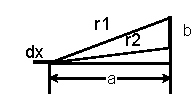
\includegraphics[width=50mm]{inc/img/mikk-1}              & \vspace{-20mm} \[ \psi_{dx, b} = \frac a2 \left[\frac{N_1(kr_2)}{r_2} - \frac{N_1(kr_1)}{r_1}\right] \]                                                                          & \vspace{-20mm} \[ \varphi_{dx, b} = \frac a2 \left(\frac{1}{r_2} - \frac{1}{r_1}\right)\] \\ \hline
			\vspace{1mm}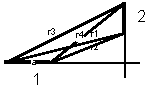
\includegraphics[width=50mm]{inc/img/mikk-2}  & \vspace{2mm} \begin{gather*} \psi_{1,2} = \frac{1}{2ka} [N_2(kr_2) + N_2(kr_3) - \\ - N_2(kr_1) - N_2(kr_4)] \end{gather*}                                                       & \vspace{5mm} \[ \varphi_{1,2} = \frac{1}{2a} (r_1 + r_4 - r_2 - r_3) \]                   \\ \hline
			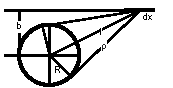
\includegraphics[width=50mm]{inc/img/mikk-3}              & \vspace{-25mm} \begin{gather*} \psi_{dx, l} = \frac{Rh}{\rho^2} \left[ \frac{\rho - R}{\rho} M(k\rho - kR) \right. \\ \left. + \frac R\rho S_1(k\rho - kR) \right] \end{gather*} & \vspace{-13.5mm} \[ \varphi_{dx, l} = \frac{Rh}{\rho^2} \]                                \\ \hline
		\end{tabular}
	\end{table}
\end{FixLineStretch}
\let\wC\relax
\let\wB\relax
\let\wA\relax

Метод дает удовлетворительные результаты, если излучающую систему
можно рассматривать как бесконечно длинную в одном направлении.
Практически это соответствует случаю, когда можно пренебречь излучением
и поглощением днищ цилиндрического объема.

По своему принципу метод схож с зональным, поэтому обладает всё теми же недостатками.
\subsection{Метод дискретных ординат}

\subsection{Дискретно-лучевой метод}

\def\wA{5mm}
\def\wB{28mm}
\def\wC{23mm}
\def\wD{23mm}
\def\wE{23mm}
\def\wF{23mm}
\def\wG{23mm}
\def\wH{22mm}
\def\wI{22mm}
\def\wJ{22mm}
\begin{FixLineStretch}
\begin{sidewaystable}
	\small
	\caption{Сравнительный анализ существующих методов моделирования световых полей}
	\label{tbl:existing-modeling-methods}
	\begin{tabular}{|p{\wA}|p{\wB}|p{\wC}|p{\wD}|p{\wE}|p{\wF}|p{\wG}|p{\wH}|p{\wI}|p{\wJ}|}
		\hline
		\TableHeader{\wA}{№} & \TableHeader{\wB}{Метод}                                                                                & \TableHeader{\wC}{Учёт излучения плазмы источника из объёма} & \TableHeader{\wD}{Учёт неоднородного распределения параметров плазмы по объему} & \TableHeader{\wE}{Нахождение распределения поглощённой мощности по объёму плазмы} & \TableHeader{\wF}{Использование параллельных алгоритмов} & \TableHeader{\wG}{Возможность применения метода для построения замкнутых систем моделирования} & \TableHeader{\wH}{Универсальность подходов для расчёта систем с плазмой произвольной оптической плотности} & \TableHeader{\wI}{Отсутствие вероятностного розыгрыша лучей} & \TableHeader{\wJ}{Доступность ПМО и ЭВМ} \\ \hline
		1                    & \everypar{\hspace*{0pt}} Зональный \cite{radiation-heat-transfer}                                       & Нет                                                          & Нет                                                                             & Нет                                                                               & Да                                                       & Нет                                                                                            & Нет                                                                                                        & Да                                                           & Нет                                      \\ \hline
		2                    & \everypar{\hspace*{0pt}} Обобщённых угловых коэффициентов \cite{encyclopedia-of-low-temperature-plasma} & Нет                                                          & Нет                                                                             & Нет                                                                               & Да                                                       & Нет                                                                                            & Нет                                                                                                        & Да                                                           & Нет                                      \\ \hline
		3                    & \everypar{\hspace*{0pt}} Дискретных ординат \cite{surzhikov}                                            & Да                                                           & Нет                                                                             & Нет                                                                               & Да                                                       & Да                                                                                             & Нет                                                                                                        & Да                                                           & Нет                                      \\ \hline
		4                    & \everypar{\hspace*{0pt}} Дискретно-лучевой \cite{gradov-dissertation}                                   & Да                                                           & Да                                                                              & Нет                                                                               & Нет                                                      & Да                                                                                             & Да                                                                                                         & Нет                                                          & Да                                       \\ \hline
	\end{tabular}
\end{sidewaystable}
\end{FixLineStretch}
\let\wJ\relax
\let\wI\relax
\let\wH\relax
\let\wG\relax
\let\wF\relax
\let\wE\relax
\let\wD\relax
\let\wC\relax
\let\wB\relax
\let\wA\relax

\section{Формализация задачи}


\let\wF\relax